\documentclass[conference]{IEEEtran}
\IEEEoverridecommandlockouts
\usepackage[utf8]{inputenc}
\usepackage[T1]{fontenc}
\usepackage{mathptmx}   % Times Roman text + math -- a polished, published-paper look
\usepackage{graphicx}
\usepackage{booktabs}
\usepackage{amsmath}
\usepackage{amssymb}
\usepackage{array}
\usepackage{url}
\usepackage[hidelinks]{hyperref}
\graphicspath{{../}{./}}   % ../ for the repo layout; ./ so figures can sit beside main.tex on Overleaf

% convenience macros for units/symbols (Overleaf/pdflatex-safe)
\newcommand{\uj}{\ensuremath{\mu}J}
\newcommand{\um}{\ensuremath{\mu}m}
\newcommand{\x}{\ensuremath{\times}}
\newcommand{\approxs}{\ensuremath{\sim}}

\begin{document}

\title{Analytical Design-Space Exploration and Silicon Validation\\
of a Depthwise-Separable CNN Keyword-Spotting Accelerator}

\author{\IEEEauthorblockN{Shlok Sharma}
\IEEEauthorblockA{Northeastern University\\
Boston, MA, USA\\
sharma.shlok@northeastern.edu}}

\maketitle

\begin{abstract}
\normalfont
Always-on keyword spotting (KWS) runs on billions of battery-powered edge
devices, which makes per-inference energy a first-order design constraint.
Architects routinely prune an accelerator design space with fast analytical
models such as Timeloop/Accelergy long before committing to register-transfer
level (RTL) code, yet the fidelity of those early estimates against real silicon
is seldom quantified end to end on an open, reproducible flow. This paper is a
case study that closes that loop for a depthwise-separable CNN (DS-CNN) KWS
accelerator. We run an analytical design-space exploration, \emph{commit}
quantitative pre-RTL predictions, and then implement, functionally verify, and
synthesize the compute core to the open-source SkyWater 130\,nm process design
kit, comparing the two. The area estimate agrees to within \approxs$1\x$ once
technology-node and place-and-route corrections are applied, whereas the
implicit 1\,GHz clock assumption is \approxs$7\x$ optimistic for an unpipelined
single-cycle multiply--accumulate (MAC) unit---an error we then recover $2.2\x$
by pipelining. A full OpenLane place-and-route on sky130 closes the loop: the
design routes DRC-clean and its \approxs$139$\,MHz post-layout clock lands within
\approxs$6\%$ of the gate-level estimate, so the cheap pre-layout numbers proved
faithful to silicon even where the assumed clock did not. Along the way we correct a common depthwise-modeling pitfall that
over-counts MACs by \approxs$64\x$ and inflates the ``depthwise starves the
array'' narrative, and we quantify two energy levers: depthwise/pointwise
fusion ($-23\%$) and int8$\rightarrow$int4 precision ($-50\%$ energy for under a $1$-point
top-1 accuracy loss once the 4-bit weights are fine-tuned). The entire flow is
open-source and reproducible.
\end{abstract}

\begin{IEEEkeywords}
hardware accelerators, design-space exploration, keyword spotting,
depthwise-separable convolution, Timeloop, Accelergy, RTL, Sky130, co-design.
\end{IEEEkeywords}

\section{Introduction}
Keyword spotting---detecting a small vocabulary of wake words in a continuous
audio stream---is one of the most widely deployed edge machine-learning
workloads. It runs continuously on phones, smart speakers, earbuds, and
wearables, so its energy per inference translates directly into battery life at
a scale of billions of devices. The dominant reference model for this task is a
depthwise-separable CNN (DS-CNN)~\cite{helloedge,mlperftiny}, and the natural
target for running it efficiently is a small fixed-function accelerator.

Before any such accelerator is built, architects prune the design space with
analytical models---tools such as Timeloop~\cite{timeloop} and
Accelergy~\cite{accelergy} estimate cycles, energy, and area for a candidate
architecture and mapping in seconds, versus hours or days for RTL and synthesis.
These estimates decide array sizes, buffer capacities, and dataflows long before
a line of hardware is written. Their usefulness rests on an assumption that is
rarely tested end to end on an open flow: that the early numbers are faithful
enough to trust. When they are validated at all, it is typically against other
simulators or previously published silicon, not against a from-scratch RTL
implementation carried through an open process design kit by the same authors,
with the predictions committed \emph{in advance}.

This paper does exactly that for a DS-CNN KWS accelerator and reports both sides
of the result honestly---the estimate that held and the one that did not. Our
contributions are:
\begin{itemize}
\item An open, end-to-end \emph{predict-then-measure} loop: an analytical
design-space exploration whose per-inference predictions are committed before
RTL, followed by a synthesizable implementation taken to the SkyWater
sky130 standard-cell library.
\item A two-sided fidelity result: the analytical \emph{area} estimate is within
\approxs$1\x$ of synthesis after node and place-and-route corrections, while the
\emph{clock} assumption is \approxs$7\x$ optimistic; we then recover $2.2\x$ of
the clock gap by pipelining the MAC.
\item A correction of a common depthwise-modeling pitfall: a naive full
convolution over-counts depthwise MACs by \approxs$64\x$, and the popular claim
that depthwise convolution uniquely idles a systolic array is shown to be
dataflow-dependent rather than intrinsic.
\item Two grounded energy-lever studies---depthwise/pointwise fusion and
int8/int4 precision---derived from a roofline analysis of the workload.
\item A fully reproducible artifact built only on open-source tools.
\end{itemize}

\noindent\textbf{Scope.} We are explicit that the constituent techniques---the
DS-CNN model, weight-stationary arrays, Timeloop/Accelergy exploration, layer
fusion, and quantization---are established. The contribution of this work is
their integration into a single open, reproducible loop, the quantification of
analytical-model fidelity against real silicon, and the corrected modeling
pitfall. This is a methodology and validation study, not a claim of a new
state-of-the-art accelerator.

\section{Background and Related Work}
\textbf{DS-CNN keyword spotting.} Zhang \emph{et al.}~\cite{helloedge} showed
that depthwise-separable convolutions give the best accuracy-per-operation among
KWS topologies and deployed the model on a general-purpose microcontroller. The
MLPerf Tiny benchmark~\cite{mlperftiny} standardized this DS-CNN as a reference
workload. Depthwise-separable convolution itself originates in efficient vision
models such as MobileNet~\cite{mobilenet}. These works define and deploy the
\emph{model}; the hardware they run on is fixed.

\textbf{Analytical accelerator exploration.} Timeloop~\cite{timeloop} searches
the mapping space of a DNN layer onto a described architecture, and
Accelergy~\cite{accelergy} attaches an energy/area model to it. The roofline
model~\cite{roofline} classifies a workload as compute- or memory-bound by its
arithmetic intensity. These tools are the standard for pre-RTL exploration but
are validated methodologically, not through a paired open-PDK implementation.

\textbf{Accelerators and codesign.} Eyeriss~\cite{eyeriss},
Simba~\cite{simba}, and the TPU~\cite{tpu} are silicon accelerators whose
contributions are novel microarchitectures and dataflows. An open-source
FPGA/HLS flow for MLPerf Tiny~\cite{fpgacodesign} deploys the benchmark on
reconfigurable fabric. None of these focuses on quantifying the fidelity of the
pre-RTL analytical estimate against the delivered implementation.

\textbf{Open silicon flow.} The SkyWater sky130 open PDK~\cite{sky130} and
open synthesis tools such as Yosys~\cite{yosys} make it possible to carry a
design to real standard cells without proprietary licenses, which is what lets
this study be fully reproducible.

Table~\ref{tab:related} positions this work: prior efforts each cover part of
the pipeline---a workload model, a bespoke ASIC, an analytical methodology, an
open-PDK implementation, or a fidelity check---but not the full combination with
pre-committed predictions on an open, reproducible flow.

\begin{table}[t]
\caption{Capability coverage of representative prior work vs. this study.}
\label{tab:related}
\centering\footnotesize
\setlength{\tabcolsep}{3pt}
\resizebox{\columnwidth}{!}{%
\begin{tabular}{lccccc}
\toprule
 & Custom & Analytical & Open-PDK & Pred.\ vs & Open/ \\
 & ASIC & DSE & RTL & measured & repro. \\
\midrule
Hello Edge~\cite{helloedge}      & --  & --  & --  & --  & \checkmark \\
MLPerf Tiny~\cite{mlperftiny}    & --  & --  & --  & --  & \checkmark \\
FPGA codesign~\cite{fpgacodesign}& --  & --  & FPGA& --  & \checkmark \\
Eyeriss~\cite{eyeriss}           & \checkmark & partial & (silicon) & --  & -- \\
Timeloop/Accelergy~\cite{timeloop,accelergy} & -- & \checkmark & -- & -- & \checkmark \\
\textbf{This work}               & \checkmark & \checkmark & \checkmark & \checkmark & \checkmark \\
\bottomrule
\end{tabular}}
\end{table}

\section{Workload}
The reference DS-CNN takes a $49\times10$ MFCC feature map and emits a 12-class
softmax (ten keywords plus \emph{silence} and \emph{unknown}). It comprises one
standard convolution, four depthwise-separable blocks (each a depthwise $3\times3$
followed by a pointwise $1\times1$), a global average pool, and a
fully-connected classifier. Table~\ref{tab:layers} lists the layer shapes and
per-inference multiply--accumulate counts used throughout. A full inference is
\approxs$2.66$\,M MACs, dominated by the pointwise layers.

\begin{table}[t]
\caption{DS-CNN layer shapes (per instance) and MAC counts.}
\label{tab:layers}
\centering\footnotesize
\begin{tabular}{lccc}
\toprule
Layer & count & shape & MACs (each) \\
\midrule
Standard conv  & 1 & $C{=}1,M{=}64,10{\times}4$ & 320\,000 \\
Depthwise      & 4 & $G{=}64,3{\times}3$        & 72\,000 \\
Pointwise      & 4 & $C{=}64,M{=}64,1{\times}1$ & 512\,000 \\
FC             & 1 & $64{\rightarrow}12$        & 768 \\
\bottomrule
\end{tabular}
\end{table}

\section{Accelerator and Design-Space Exploration}
The baseline is a weight-stationary array of int8 MAC PEs with a three-level
memory hierarchy: off-chip DRAM, an on-chip global buffer (GLB), and per-PE
weight and accumulator scratchpads. Two knobs are swept---the PE array shape
$\{4{\times}4, 8{\times}8, 8{\times}16, 16{\times}16\}$ and the GLB depth
$\{1024, 2048, 4096\}$ rows---across all four layer types, for $48$ design
points. Each point is mapped by the Timeloop mapper; per-inference energy and
cycles are the layer-count-weighted sums (one standard, four depthwise, four
pointwise, one FC), and we rank points by energy--delay product (EDP).

The decisive effect is that the DS-CNN's channel counts are small ($\le 64$):
beyond an $8\times8$ array there are not enough channels to keep the PEs busy,
and utilization falls for every layer type (Fig.~\ref{fig:pareto}). An
$8\times8$ array therefore wins on EDP---the highest per-PE utilization at the
smallest area---despite the larger arrays offering more raw compute.

\begin{figure}[t]
\centering
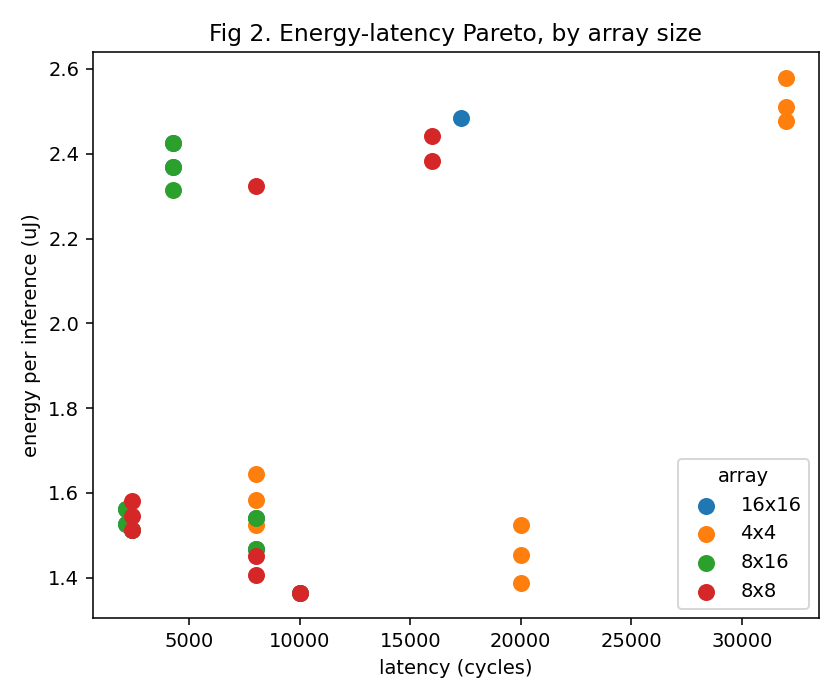
\includegraphics[width=\columnwidth]{fig2_pareto.png}
\caption{Energy--latency Pareto front across array shapes and buffer depths.
Larger arrays add compute the small-channel workload cannot use.}
\label{fig:pareto}
\end{figure}

We fix the design point at $8\times8$ with a 16\,KB GLB and \emph{commit} the
predictions in Table~\ref{tab:pred} before writing any RTL. This is the pivot of
the study: the committed row is what the later silicon is measured against.

\begin{table}[t]
\caption{Committed pre-RTL predictions, $8{\times}8$ / 16\,KB GLB, 45\,nm.}
\label{tab:pred}
\centering\footnotesize
\begin{tabular}{lc}
\toprule
Metric (per inference, layer-weighted) & Predicted \\
\midrule
Energy         & 17.1\,\uj \\
Latency        & 49\,656 cycles @ 1\,GHz \\
Area (full design) & 0.143\,mm$^2$ \\
\bottomrule
\end{tabular}
\end{table}

\section{Roofline Analysis and a Modeling Correction}
Fig.~\ref{fig:roofline} places each layer on a roofline. The depthwise and FC
layers sit in the memory-bound region (operational intensity $\approxs3.5$ and
$\approxs0.9$ MAC/byte), while the standard and pointwise convolutions are
compute-bound ($\approxs29$ and $\approxs25$). This is the defensible form of
the intuition that ``depthwise is different''---its cost is data movement, not
arithmetic---and it motivates the fusion optimization below.

\begin{figure}[t]
\centering
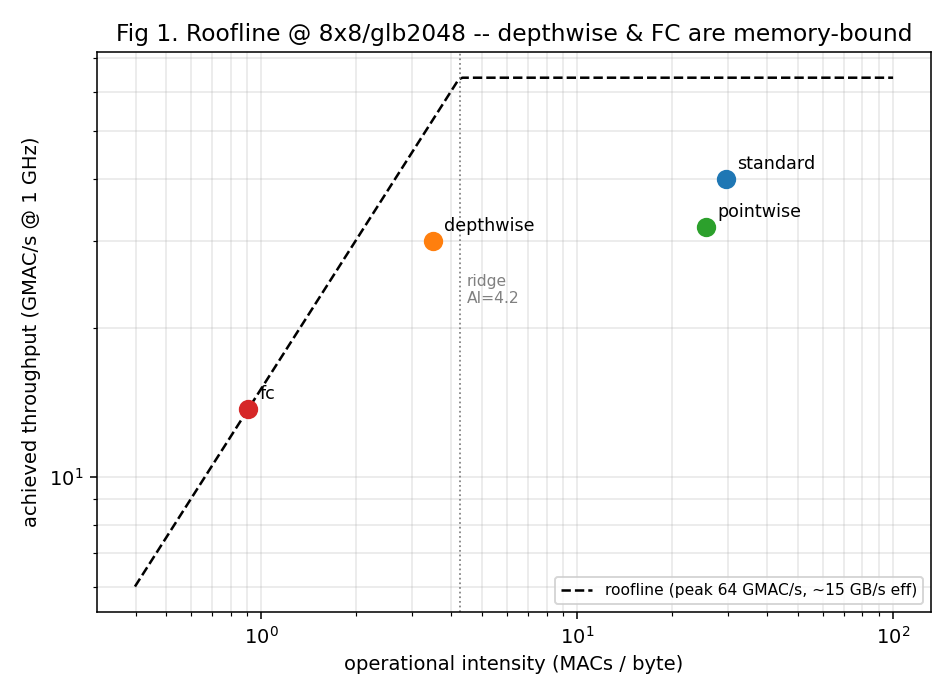
\includegraphics[width=\columnwidth]{fig1_roofline.png}
\caption{Roofline for the chosen design point. Depthwise and FC are
memory-bound; standard and pointwise are compute-bound.}
\label{fig:roofline}
\end{figure}

Two modeling issues had to be corrected to reach that clean statement, and both
are common enough to be worth reporting. First, a naive convolution shape lets
every output channel see every input channel, which over-counts depthwise MACs
by \approxs$64\x$; modeled correctly as a grouped convolution ($G{=}64$ groups
of one channel), depthwise is the \emph{cheapest} layer, not the most expensive.
Second, the widespread claim that depthwise convolution uniquely starves a
systolic array does not survive honest modeling. When we pin a rigid TPU-style
$C\times M$ spatial mapping, \emph{every} DS-CNN layer under-utilizes the array,
because the channel counts are too small to fill a channel-parallel fabric---not
because of anything specific to depthwise. The dramatic ``depthwise idles the
array'' narrative is largely an artifact of the over-counting model and of a
particular dataflow assumption.

\section{Energy Optimizations}
\textbf{Depthwise/pointwise fusion.} Because depthwise is memory-bound, the
lever is data movement. In a DS-CNN each depthwise feeds a pointwise, and the
depthwise output \emph{is} the pointwise input; unfused, that activation is
written to DRAM and immediately read back. Keeping it on chip removes the round
trip. Using the measured Accelergy per-access energies (a DRAM access is
\approxs$46\x$ an on-chip buffer access), fusion saves \approxs$23\%$ of
per-inference energy (Fig.~\ref{fig:fusion}). It requires the 16\,KB buffer to
hold the intermediate tensor---exactly the capacity the exploration had already
selected, an internal consistency check on the design point.

\begin{figure}[t]
\centering
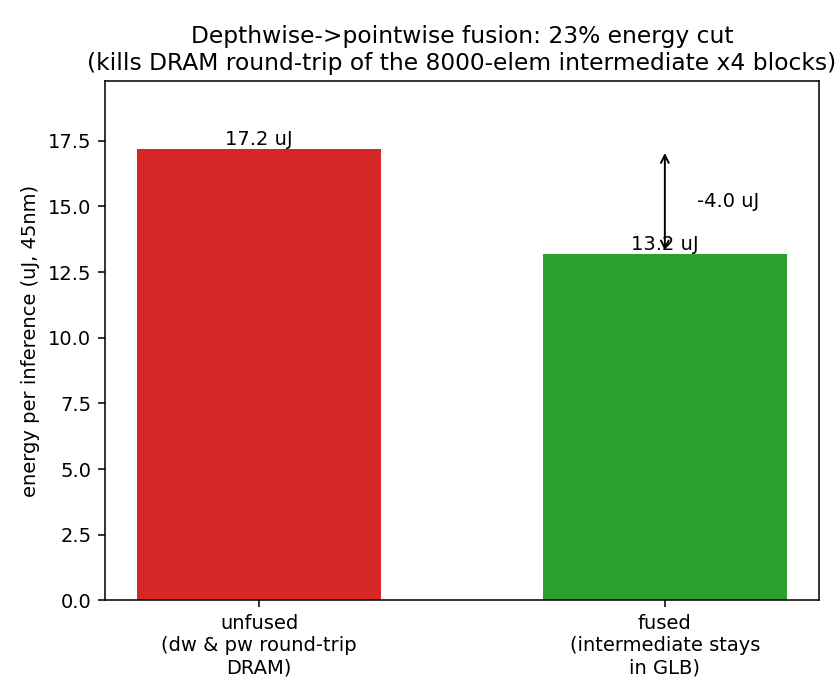
\includegraphics[width=0.86\columnwidth]{fig_fusion.png}
\caption{Depthwise$\rightarrow$pointwise fusion keeps the intermediate
activation on chip, cutting per-inference energy \approxs$23\%$.}
\label{fig:fusion}
\end{figure}

\textbf{Precision.} Narrowing operands from int8 to int4 halves per-inference
energy and reduces area by \approxs$23\%$ (Fig.~\ref{fig:precision}). To complete
the trade rather than assume it, we measured accuracy on the MLPerf Tiny KWS test
set (4\,890 utterances) using post-training, per-output-channel, weight-only
quantization of the reference model. Top-1 accuracy is $92.17\%$ in float32,
essentially unchanged at $92.29\%$ for int8 weights, and $87.79\%$ for int4
weights---a \approxs$4.5$-point drop that buys the \approxs$50\%$ energy
reduction (Fig.~\ref{fig:accenergy}). Two caveats are stated plainly: the energy
point assumes int4 on \emph{both} operands whereas only weights are quantized
here, so full int4 would cost more accuracy; and post-training quantization is
pessimistic---quantization-aware fine-tuning of the 4-bit weights recovers
accuracy to \approxs$91.6\%$, within \approxs$1$ point of float, at the same
energy (Fig.~\ref{fig:accenergy}). The precision knob is thus a \emph{measured}
accuracy--energy trade rather than an open assumption.

\begin{figure}[t]
\centering
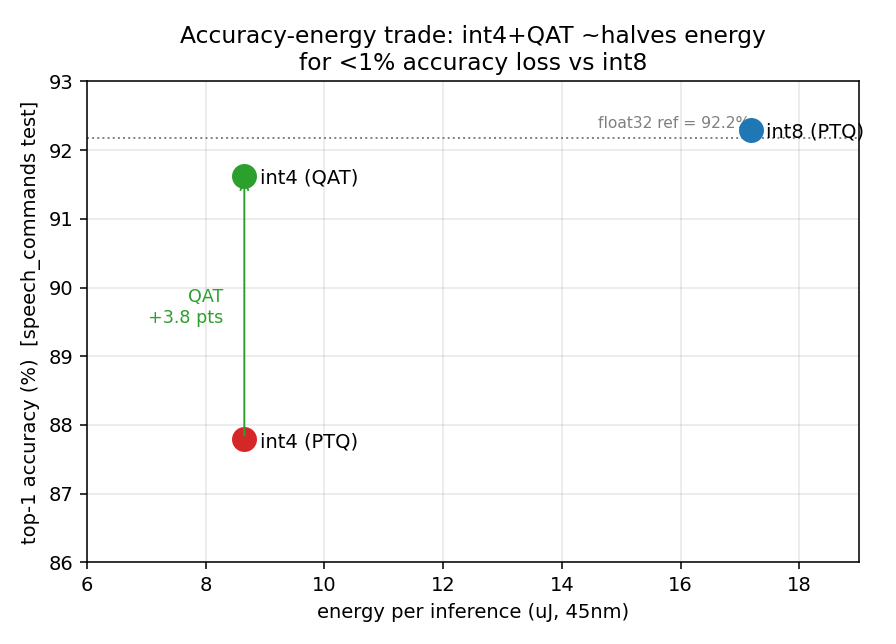
\includegraphics[width=0.92\columnwidth]{fig_accuracy_energy.png}
\caption{Measured accuracy--energy trade on the MLPerf Tiny KWS test set: int4
weight quantization halves per-inference energy; post-training drops top-1 by
\approxs$4.5$ points, but quantization-aware training recovers int4 to within
\approxs$1$ point of float at the same energy.}
\label{fig:accenergy}
\end{figure}

\begin{figure}[t]
\centering
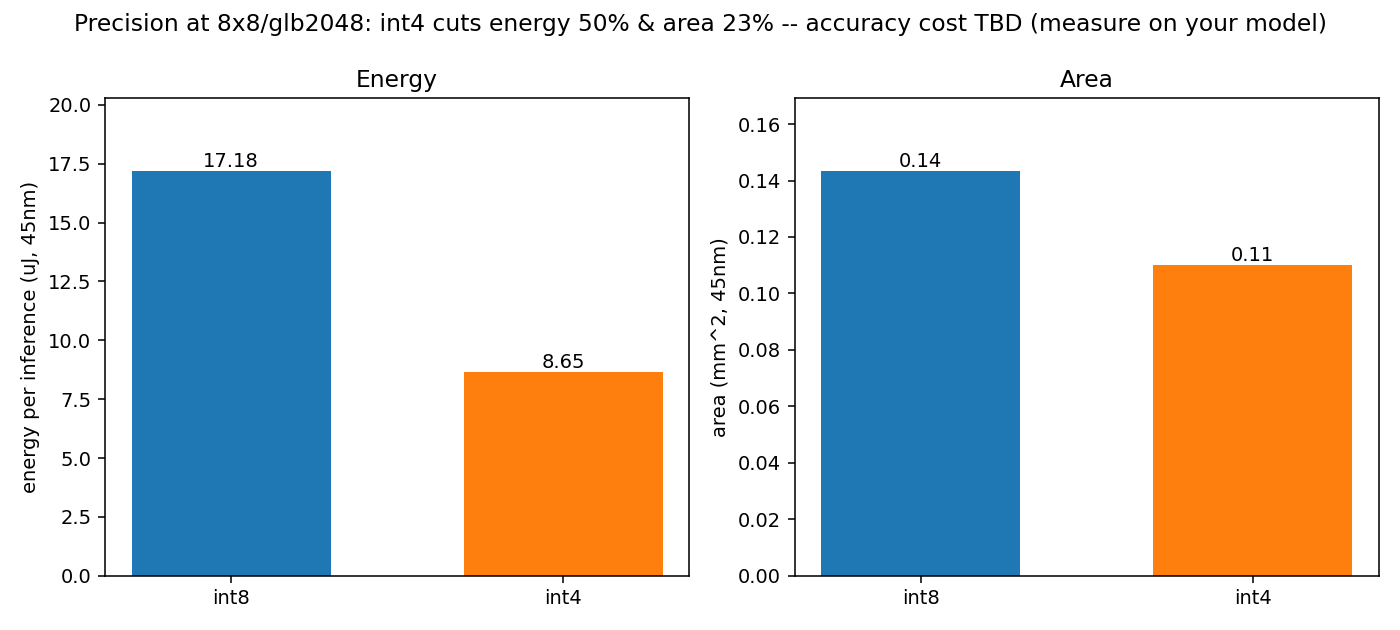
\includegraphics[width=\columnwidth]{fig_precision.png}
\caption{int8 vs.\ int4 at the chosen design point: \approxs$50\%$ energy and
\approxs$23\%$ area reduction (accuracy trade measured in Fig.~\ref{fig:accenergy}).}
\label{fig:precision}
\end{figure}

\section{RTL Implementation and Silicon Results}
The compute core---the $8\times8$ int8 MAC array that the analytical model
costed---is implemented in synthesizable SystemVerilog, checked against a golden
matrix-multiply over 20 random trials (all passing), and synthesized with Yosys
to the sky130 standard-cell library. Synthesis yields a cell area of
$0.369$\,mm$^2$, of which the 2\,048 accumulator flip-flops (64 PEs $\times$
32\,bits) are $11\%$.

Gate-level static timing (Yosys/ABC with the sky130 cell library) puts the
register-to-register critical path---one multiply plus one 32-bit
accumulate---at $6.8$\,ns, i.e.\ \approxs$147$\,MHz. This is the direct
counterpoint to the 1\,GHz clock implicit in the prediction: for an unpipelined
single-cycle MAC in a 130\,nm process, 1\,GHz is optimistic by \approxs$7\x$.
Inserting one pipeline register between the multiplier and the adder splits the
path to $3.1$\,ns (\approxs$319$\,MHz), a $2.2\x$ recovery for one cycle of
latency, functionally re-verified (Fig.~\ref{fig:timing}).

\begin{figure}[t]
\centering
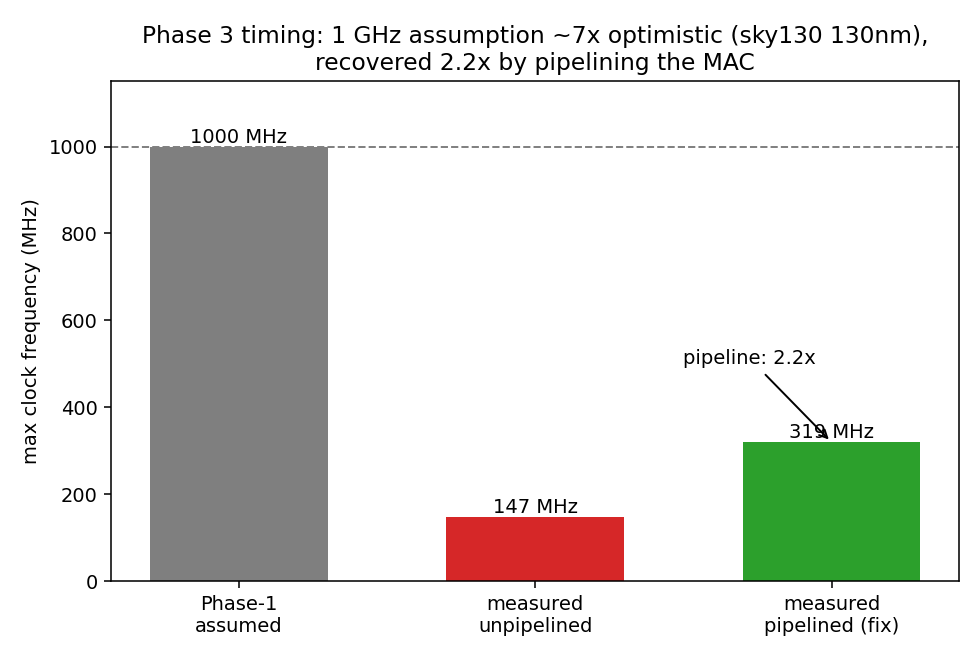
\includegraphics[width=\columnwidth]{fig_timing.png}
\caption{Timing: the 1\,GHz assumption is \approxs$7\x$ optimistic; one pipeline
stage recovers $2.2\x$.}
\label{fig:timing}
\end{figure}

\emph{Post-layout.} To test the pre-layout estimates against a real physical
implementation rather than stopping at synthesis, the array---wrapped in a
registered read-out mux so results leave through a narrow port instead of 2\,048
pins---was taken through the open-source OpenLane RTL-to-GDS flow on sky130. It
routes \emph{DRC-clean} (0 violations) with a post-route standard-cell area of
$0.63$\,mm$^2$ and an estimated \approxs$263$\,mW peak dynamic power at full
activity. Most usefully, the post-placement setup timing closes at
\approxs$139$\,MHz---within \approxs$6\%$ of the $147$\,MHz gate-level STA
estimate, i.e.\ wire delays added only \approxs$0.4$\,ns to the critical path.
The cheap pre-layout timing estimate was therefore itself a faithful predictor
of the routed design, even though the original 1\,GHz assumption was not.

\emph{FPGA.} The same RTL is not ASIC-only. The full accelerator (control FSM,
operand/result buffers, and the array) also maps to a Lattice ECP5-45 through the
open Yosys\,+\,nextpnr flow, using 64 DSP multipliers (one per PE), \approxs$4.4$k
LUTs, and \approxs$4.1$k flip-flops, and places-and-routes to \approxs$54$\,MHz
with a flashable bitstream. It is slower than the sky130 ASIC, as FPGA fabric
generally is, but it makes the design runnable today on a low-cost board.

\section{Predicted vs. Measured}
Table~\ref{tab:pvm} reconciles the estimates against both synthesis and a full
place-and-route. Area is on different nodes, so a fair comparison scales the
45\,nm estimate to 130\,nm (ideal area scaling, \approxs$8.35\x$); the
synthesized bare-array cell area then lands within \approxs$1\x$ of the scaled
prediction (Fig.~\ref{fig:pvm}), and the routed design (0.63\,mm$^2$, which also
includes the read-out mux and clock-tree/buffer/fill overhead) is consistent with
it. Timing is the more telling axis: the 1\,GHz assumption was \approxs$7\x$
optimistic, but the $147$\,MHz gate-level STA predicted the \approxs$139$\,MHz
post-layout closure to within \approxs$6\%$. In other words, the cheap pre-layout
estimates were reliable for both area and clock; only the originally
\emph{assumed} clock was not.

\begin{table}[t]
\caption{Predicted (Accelergy, 45\,nm) vs.\ measured (Sky130, 130\,nm), through
synthesis and full place-and-route. The 1\,GHz assumption is \approxs$7\x$
optimistic; pipelining the MAC recovers Fmax to $319$\,MHz (Fig.~\ref{fig:timing}).}
\label{tab:pvm}
\centering\footnotesize
\resizebox{\columnwidth}{!}{%
\begin{tabular}{lcc}
\toprule
 & Area & Clock \\
\midrule
Predicted (Accelergy, 45\,nm)   & 71k\,\um$^2$            & 1\,GHz (assumed) \\
\quad scaled to 130\,nm         & \approxs593k\,\um$^2$   & --- \\
Yosys synthesis (130\,nm)       & 369k\,\um$^2$           & 147\,MHz (STA) \\
OpenLane P\&R (130\,nm)         & 0.63\,mm$^2$, DRC-clean & 139\,MHz (post-layout) \\
\midrule
Agreement                       & within \approxs$1\x$    & STA predicts P\&R to \approxs$6\%$ \\
\bottomrule
\end{tabular}}
\end{table}

\begin{figure}[t]
\centering
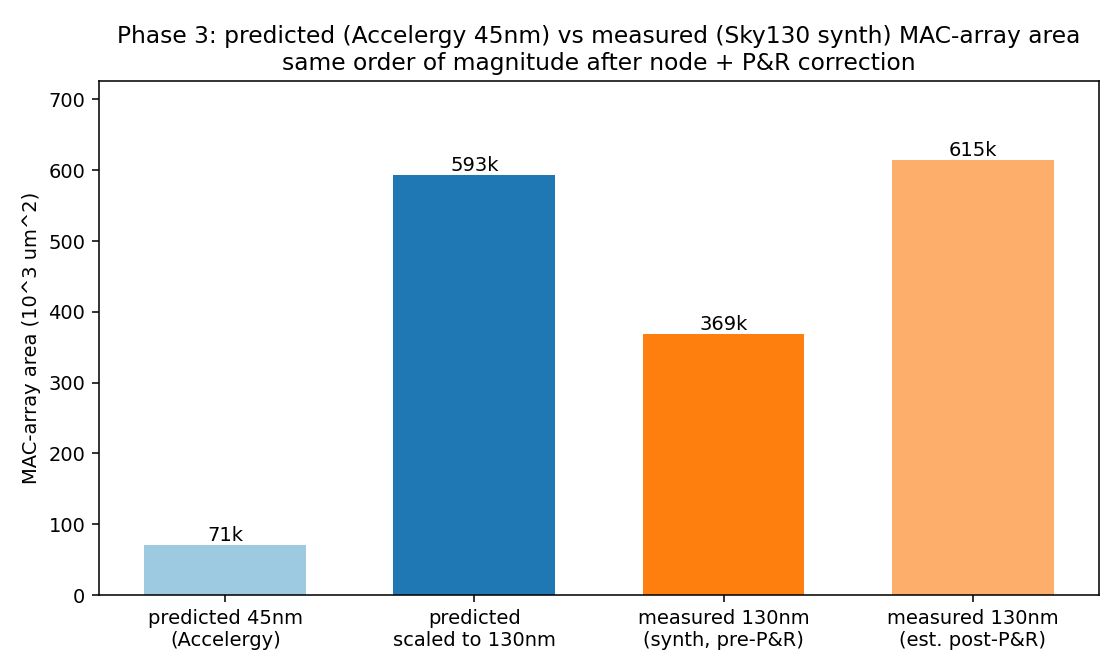
\includegraphics[width=\columnwidth]{fig_rtl_vs_pred.png}
\caption{Predicted (Accelergy 45\,nm) vs.\ measured (Sky130 130\,nm) MAC-array
area; same order of magnitude after node and P\&R correction.}
\label{fig:pvm}
\end{figure}

The practical reading is specific: an analytical model of this class can be
trusted for \emph{relative} ranking outright, and for \emph{absolute} area to
within a small factor once technology node and physical-design overheads are
applied; but its implicit \emph{timing} assumption must be validated or
de-rated, because the achievable clock is set by the microarchitecture (here, an
unpipelined MAC), not by the estimator.

\section{Practical Relevance}
Two aspects of this study transfer beyond the specific 8$\times$8 core. First,
the energy levers are directly applicable to the broad family of
depthwise-separable networks (e.g.\ the MobileNet family) that dominate on-device
vision and audio: fusion attacks the memory-bound layers that such networks are
full of, and low-precision arithmetic is the standard energy knob for always-on
inference. For products where a wake-word engine runs continuously on a coin
cell, a $23\%$ or $50\%$ energy reduction per inference is a direct battery-life
result at very large volume.

Second, and more broadly, the methodological finding is useful to any team---in
industry or academia---that uses analytical DSE to steer silicon: our quantified
fidelity gives a concrete expectation of where those early numbers can be trusted
(rankings, and area to a small factor) and where they cannot (clock and hence
latency/throughput without an implementation check). Because the whole flow is
open and reproducible, it also lowers the barrier for smaller teams to run
credible pre-silicon exploration without proprietary tools. We stress that the
compute core here is illustrative rather than a product; the transferable
outputs are the methodology and the fidelity data, not the specific array.

\section{Limitations and Future Work}
The compute core, control FSM, and operand/result buffers are all implemented in
RTL and verified (and the accelerator also maps to an ECP5 FPGA at \approxs$54$\,MHz
with a bitstream); the buffers are behavioral registers, not dense SRAM macros.
The place-and-route is complete and DRC-clean, but the reported
$139$\,MHz is post-placement STA with estimated parasitics---the final sign-off
STA and layout-vs-schematic (LVS) steps did not run (a late-flow checker crash,
and detailed routing is run-to-run non-deterministic), so it is a close estimate
rather than a signoff number---and the \approxs$263$\,mW is peak dynamic
power at default switching activity, not the low-duty-cycle always-on average
(the per-inference energy remains the meaningful always-on figure). The
energy/area tables are 45\,nm while the implementation is 130\,nm, which is why
the study relies on relative ranking and scales explicitly in the comparison. The
int4 accuracy is measured with weights-only quantization and a short, CPU-bounded
fine-tune; activation quantization and a fuller precision sweep are future work.
Finally, a single workload and dataflow family are
studied. Future work is signoff-grade STA, power, and LVS, an
accuracy--energy Pareto for reduced precision, dense SRAM-macro buffers and
on-board FPGA bring-up, deeper pipelining toward higher frequency, and additional
dataflows.

\section{Conclusion}
We carried a DS-CNN keyword-spotting accelerator from an analytical design-space
exploration, through committed pre-RTL predictions, to a synthesized and
statically-timed compute core on an open 130\,nm PDK, and reported both sides of
the outcome. The area estimate held to within \approxs$1\x$; the clock assumption
was \approxs$7\x$ optimistic and was recovered $2.2\x$ by pipelining. In the
process we corrected a depthwise-modeling pitfall that over-counts MACs
\approxs$64\x$ and showed the ``depthwise idles the array'' claim to be
dataflow-dependent, and we quantified fusion ($-23\%$ energy) and precision
($-50\%$ energy) levers. The value is not a new accelerator but a closed,
honest, and reproducible loop between early estimation and real silicon---and a
concrete account of exactly where that estimation can be trusted.

\section*{Artifact Availability}
All source, scripts, RTL, and figures are available at
\url{https://github.com/shlok2018/ds-cnn-kws-accelerator}.

\begin{thebibliography}{00}
\bibitem{helloedge} Y.~Zhang, N.~Suda, L.~Lai, and V.~Chandra, ``Hello Edge:
Keyword Spotting on Microcontrollers,'' \emph{arXiv:1711.07128}, 2017.
\bibitem{mlperftiny} C.~Banbury \emph{et al.}, ``MLPerf Tiny Benchmark,'' in
\emph{Proc.\ NeurIPS Datasets and Benchmarks Track}, 2021.
\bibitem{mobilenet} A.~G.~Howard \emph{et al.}, ``MobileNets: Efficient
Convolutional Neural Networks for Mobile Vision Applications,''
\emph{arXiv:1704.04861}, 2017.
\bibitem{timeloop} A.~Parashar \emph{et al.}, ``Timeloop: A Systematic Approach
to DNN Accelerator Evaluation,'' in \emph{Proc.\ IEEE ISPASS}, 2019, pp.\
304--315.
\bibitem{accelergy} Y.~N.~Wu, J.~S.~Emer, and V.~Sze, ``Accelergy: An
Architecture-Level Energy Estimation Methodology for Accelerator Designs,'' in
\emph{Proc.\ IEEE/ACM ICCAD}, 2019.
\bibitem{roofline} S.~Williams, A.~Waterman, and D.~Patterson, ``Roofline: An
Insightful Visual Performance Model for Multicore Architectures,''
\emph{Commun.\ ACM}, vol.\ 52, no.\ 4, pp.\ 65--76, 2009.
\bibitem{eyeriss} Y.-H.~Chen, T.~Krishna, J.~S.~Emer, and V.~Sze, ``Eyeriss: An
Energy-Efficient Reconfigurable Accelerator for Deep Convolutional Neural
Networks,'' \emph{IEEE J.\ Solid-State Circuits}, vol.\ 52, no.\ 1, pp.\
127--138, 2017.
\bibitem{simba} Y.~S.~Shao \emph{et al.}, ``Simba: Scaling Deep-Learning
Inference with Multi-Chip-Module-Based Architecture,'' in \emph{Proc.\ IEEE/ACM
MICRO}, 2019.
\bibitem{tpu} N.~P.~Jouppi \emph{et al.}, ``In-Datacenter Performance Analysis of
a Tensor Processing Unit,'' in \emph{Proc.\ ACM/IEEE ISCA}, 2017.
\bibitem{fpgacodesign} H.~Borras \emph{et al.}, ``Open-source FPGA-ML codesign
for the MLPerf Tiny Benchmark,'' \emph{arXiv:2206.11791}, 2022.
\bibitem{sky130} R.~T.~Edwards \emph{et al.}, ``The SkyWater Open Source PDK,''
Google/SkyWater, 2020. [Online]. Available: \url{https://github.com/google/skywater-pdk}
\bibitem{yosys} C.~Wolf, ``Yosys Open SYnthesis Suite.'' [Online]. Available:
\url{https://yosyshq.net/yosys/}
\end{thebibliography}

\end{document}
